%%%%%%%%%%%%%%%%%%%%%%%%%%%%%%%%%%%%%%%%%
% Short Sectioned Assignment
% LaTeX Template
% Version 1.0 (5/5/12)
%
% This template has been downloaded from:
% http://www.LaTeXTemplates.com
%
% Original author:
% Frits Wenneker (http://www.howtotex.com)
%
% License:
% CC BY-NC-SA 3.0 (http://creativecommons.org/licenses/by-nc-sa/3.0/)
%
%%%%%%%%%%%%%%%%%%%%%%%%%%%%%%%%%%%%%%%%%

%----------------------------------------------------------------------------------------
%	PACKAGES AND OTHER DOCUMENT CONFIGURATIONS
%----------------------------------------------------------------------------------------

\documentclass[paper=a4, fontsize=11pt]{scrartcl} % A4 paper and 11pt font size

\usepackage[T1]{fontenc} % Use 8-bit encoding that has 256 glyphs
%\usepackage{fourier} % Use the Adobe Utopia font for the document - comment this line to return to the LaTeX default
\usepackage[english]{babel} % English language/hyphenation
\usepackage{amsmath,amsfonts,amsthm} % Math packages
%\usepackage[version=3]{mhchem} % Package for chemical equation typesetting
\usepackage{siunitx} % Provides the \SI{}{} and \si{} command for typesetting SI units
\usepackage{graphicx} % Required for the inclusion of images
%\usepackage{natbib} % Required to change bibliography style to APA
\usepackage{authblk}
\usepackage{indentfirst}
\usepackage{subcaption}
\usepackage{wrapfig}
\usepackage{multirow}
\usepackage{hyperref}
\usepackage{float}
\usepackage{url}
\usepackage{booktabs}
\usepackage{times}
\usepackage{wrapfig}

\usepackage{lipsum} % Used for inserting dummy 'Lorem ipsum' text into the template

\usepackage{sectsty} % Allows customizing section commands
\allsectionsfont{\centering \normalfont\scshape} % Make all sections centered, the default font and small caps

\usepackage{geometry}
\geometry{left=2.5cm,right=2.5cm,top=2.5cm,bottom=2.5cm}

\graphicspath{{images/}{figures/}}

\usepackage{fancyhdr} % Custom headers and footers
\pagestyle{fancyplain} % Makes all pages in the document conform to the custom headers and footers
\fancyhead{} % No page header - if you want one, create it in the same way as the footers below
\fancyfoot[L]{} % Empty left footer
\fancyfoot[C]{} % Empty center footer
\fancyfoot[R]{\thepage} % Page numbering for right footer
\renewcommand{\headrulewidth}{0pt} % Remove header underlines
\renewcommand{\footrulewidth}{0pt} % Remove footer underlines
\setlength{\headheight}{13.6pt} % Customize the height of the header

\numberwithin{equation}{section} % Number equations within sections (i.e. 1.1, 1.2, 2.1, 2.2 instead of 1, 2, 3, 4)
\numberwithin{figure}{section} % Number figures within sections (i.e. 1.1, 1.2, 2.1, 2.2 instead of 1, 2, 3, 4)
\numberwithin{table}{section} % Number tables within sections (i.e. 1.1, 1.2, 2.1, 2.2 instead of 1, 2, 3, 4)

\linespread{1.2}

%\setlength\parindent{0pt} % Removes all indentation from paragraphs - comment this line for an assignment with lots of text

%----------------------------------------------------------------------------------------
%	TITLE SECTION
%----------------------------------------------------------------------------------------

\newcommand{\horrule}[1]{\rule{\linewidth}{#1}} % Create horizontal rule command with 1 argument of height

\title{	
	\normalfont \normalsize 
	\textsc{Philipps-Universitaet Marburg, The Department of Physics} \\ [25pt] % Your university, school and/or department name(s)
	\horrule{0.5pt} \\[0.4cm] % Thin top horizontal rule
	\huge Computational Physics II : Assignment 3 \\ % The assignment title
	\horrule{2pt} \\[0.5cm] % Thick bottom horizontal rule
}

\author{Houchen \textsc{Li}, Dayeon \textsc{Kang}} % Your name

\date{\normalsize\today} % Today's date or a custom date

\begin{document}

\maketitle % Print the title

%----------------------------------------------------------------------------------------
%	PROBLEM 1
%----------------------------------------------------------------------------------------

\section{Random walk with memory}

We first picked up 100000 points for \(x_0=0\), then we evaluate them for 1000 steps with memorized random walks
\begin{equation}
	x_0=0,\quad x_1=x_0+l_0,\quad\cdots,\quad x_{n+1}=x_n+l_n\quad
	\label{equ:memorized_random_walk:position}
\end{equation}
where
\begin{equation}
	l_0=\begin{cases}1 & \text{ with probability of \(0.5\) } \\ -1 & \text{ with probability of \(0.5\) }\end{cases},\quad l_n=\begin{cases}l_{n-1} & \text{ with probability of \(0.5+\varepsilon\) } \\ -l_{n-1} & \text{ with probability of \(0.5-\varepsilon\) }\end{cases}
	\label{equ:memorized_random_walk:step}
\end{equation}
for \(\varepsilon\in\left\{0.1,0.2,0.3,0.4\right\}\). The results are presented in Figure~\ref{fig:random_walk_with_memory}.\par
\begin{figure}[!htbp]
	\centering
	\begin{subfigure}[!b]{0.495\textwidth}
		\centering
		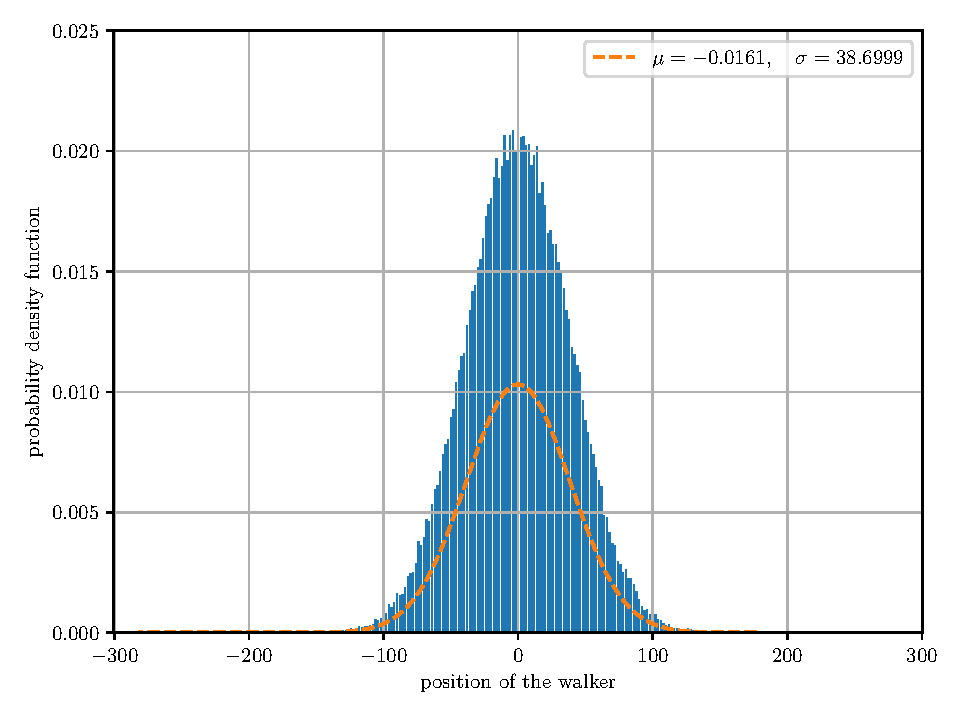
\includegraphics[width=\linewidth]{figure_1_0.pdf}
		\caption{}
	\end{subfigure}
	\begin{subfigure}[!b]{0.495\textwidth}
		\centering
		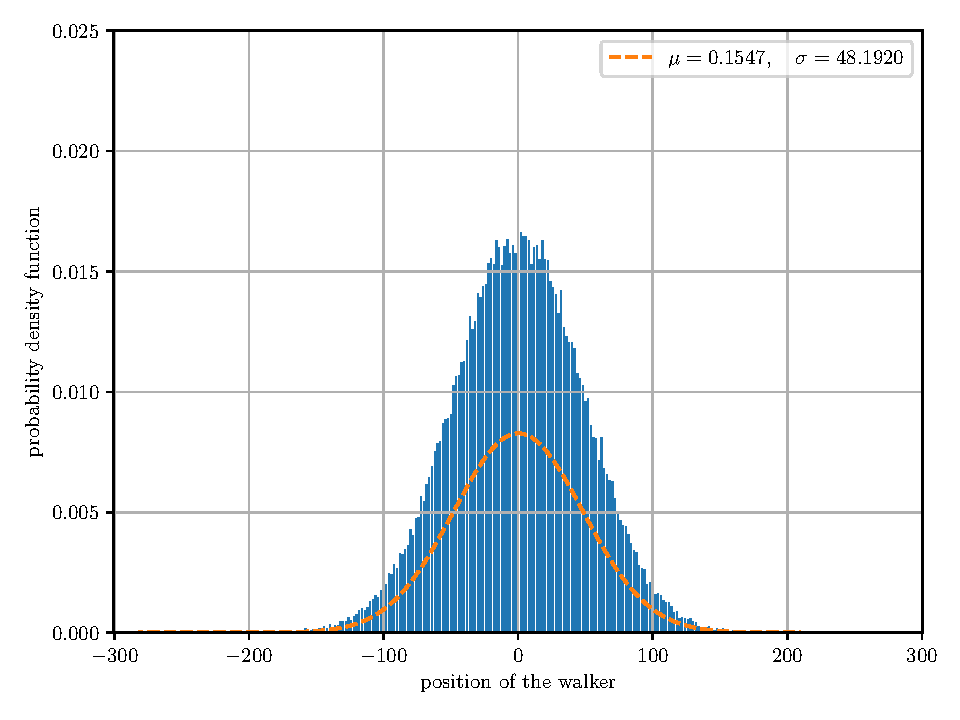
\includegraphics[width=\linewidth]{figure_1_1.pdf}
		\caption{}
	\end{subfigure}
	\begin{subfigure}[!b]{0.495\textwidth}
		\centering
		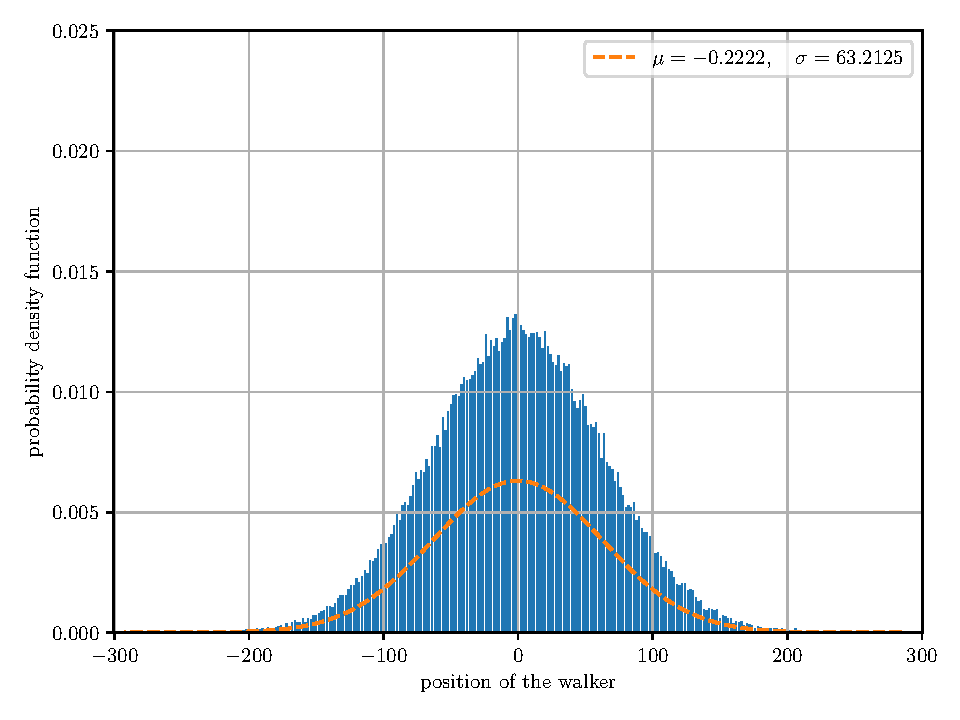
\includegraphics[width=\linewidth]{figure_1_2.pdf}
		\caption{}
	\end{subfigure}
	\begin{subfigure}[!b]{0.495\textwidth}
		\centering
		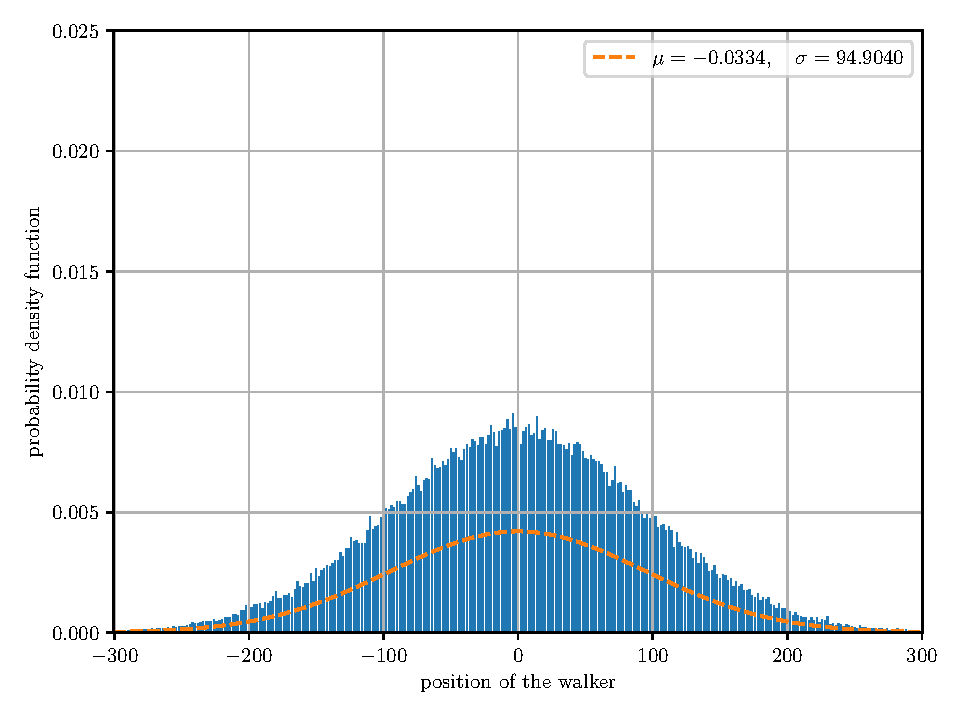
\includegraphics[width=\linewidth]{figure_1_3.pdf}
		\caption{}
	\end{subfigure}
	\caption{the statistics for the memorized random walk with \(\varepsilon=0.1,0.2,0.3,0.4\) corresponding to (a), (b), (c), (d), and their fitting curve for Gaussian distribution.}
	\label{fig:random_walk_with_memory}
\end{figure}
By using the fitting parameters \(\sigma\), the diffusion constant can be determined. 
\begin{table}[!ht]
	\centering
	\begin{tabular}{ccccc}
		\toprule
		\(\varepsilon\) & \num{0.1} & \num{0.2} & \num{0.3} & \num{0.4} \\
		\midrule
		diffusion constant \(D\) & \num{1.4977} & \num{2.3225} & \num{3.9958} & \num{9.0068} \\
		\bottomrule
	\end{tabular}
	\caption{the diffusion constant for memorized random walk with \(\varepsilon\in\left\{ 0.1,0.2,0.3,0.4 \right\}\).}
	\label{tab:random_walk_with_memory}
\end{table}
But hardly we can find the trend of the diffusion constants.\par
      
%----------------------------------------------------------------------------------------
%	PROBLEM 2
%----------------------------------------------------------------------------------------

\section{Random walks in 3d}

We first constructed the random vectors generators by following the interpretation. Our strategies go as:\par
\noindent (i) Spherical coordinates\par
The direction is given by $n = (\sin\theta  \cos\phi,\sin\theta\cos\phi, \cos\theta)$, whose probability density is determined as $d\Omega = \sin\theta d\theta\phi$. If the $\theta$ and $\phi$ are determined from uniform random number in the range of (0,$\pi$) and range (0,$2\pi$), then the directional distribution is is not uniform shown in Figure \ref{fig:2} (a).\par
To build uniform distribution of direction $ d\Omega = d\zeta d\eta\ $ where $\zeta$ and $\eta$ are uniform random variable in (-1,1).
\begin{equation}
  d\Omega = d(-\cos\theta)d\phi = d\zeta d\eta, \quad \theta = \arccos\left(-\zeta\right) \quad \& \quad \phi = \eta
\end{equation}
The results are proved to have high homogeneity which are shown in Figure \ref{fig:2} (b).\par
\vskip 1em

\noindent (ii) Sperical Volume\par
Sphere is iostropic in all direction and directional density is also  idential. So the randomly picking a point in sphere volume gives uniform direction distribution. To simulate sphere with radius 1, three random numbers $x_{i} \in (-1, 1)$ with $||x|| < 1$ are picked. The points directions are represented in Figure \ref{fig:2} (c).\par
\vskip 1em

\noindent (iii) Gaussian random distribution\par
With normally distributed random number ; $\zeta, \eta, \xi$ for cartesian coordinates, the probability density only depends on $r$. This mean for each direction the probability is identical.  The results shown in Fig \ref{fig:2} (d).\par
\begin{equation}
  d\zeta d\eta d\xi = (\frac{1}{\sigma\sqrt{2\pi}})^3e^{-\frac{x^2+ y^2+ z^2}{2\sigma^2}}dx dy dz  = (\frac{1}{\sigma\sqrt{2\pi}})^3 e^{-\frac{r^2}{2\sigma^2}} dx dy dz
\end{equation}
\vskip 1em

\begin{figure}[!ht]
	\centering
	\begin{subfigure}[b]{0.495\textwidth}
		\centering
		\includegraphics[width=\linewidth]{codes/2-0.png}
		\caption{}
	\end{subfigure}
	\begin{subfigure}[b]{0.495\textwidth}
		\centering
		\includegraphics[width=\linewidth]{codes/2-1.png}
		\caption{}
    \end{subfigure}
	\begin{subfigure}[b]{0.495\textwidth}
		\centering
		\includegraphics[width=\linewidth]{codes/2-2.png}
		\caption{}
    \end{subfigure}
    \begin{subfigure}[b]{0.495\textwidth}
		\centering
		\includegraphics[width=\linewidth]{codes/2-3.png}
		\caption{}
	\end{subfigure}
	\caption{Direction distribution with 4 different way of random variable }
	\label{fig:2}
\end{figure}

After that, in order to calculate the diffusion constant out, we plot the radius distribution of the final position. And do curve fitting with
\begin{equation}
	f\left( r \right)dr=\int_{0}^{\pi}\mathrm{d}\theta\int_{0}^{2\pi}\mathrm{d}\phi\left( \frac{1}{\sqrt{2\pi\sigma^2}} \right)^3\exp\left( -\frac{r^2}{2\sigma^2} \right)r^2\sin\theta\mathrm{d}r=\frac{\sqrt{2}}{\sqrt{\pi}\sigma^3}\exp\left( -\frac{r^2}{2\sigma^2} \right)r^2\mathrm{d}r.
	\label{equ:the_radius_distribution}
\end{equation}
The results are shown in Figure~\ref{fig:random_walks_in_3d}. By using the \(\sigma\) here, the diffusion constant are found out at \(D=0.3352\).\par
\begin{figure}[!ht]
	\centering
	\begin{subfigure}[!b]{0.495\textwidth}
		\centering
		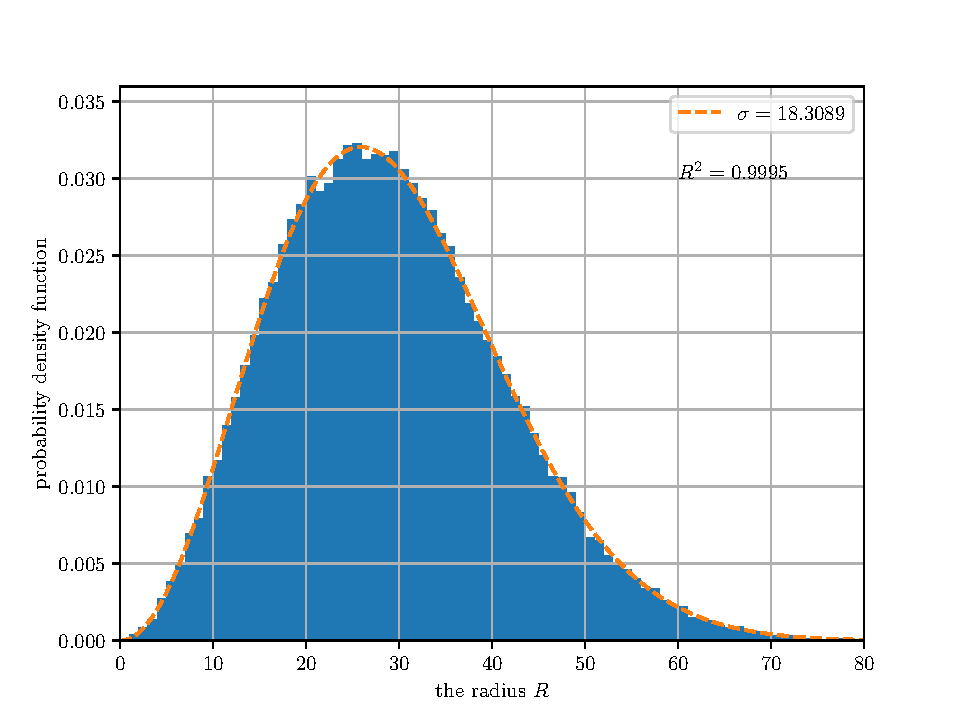
\includegraphics[width=\linewidth]{figure_2_0.pdf}
		\caption{}
	\end{subfigure}
	\begin{subfigure}[!b]{0.495\textwidth}
		\centering
		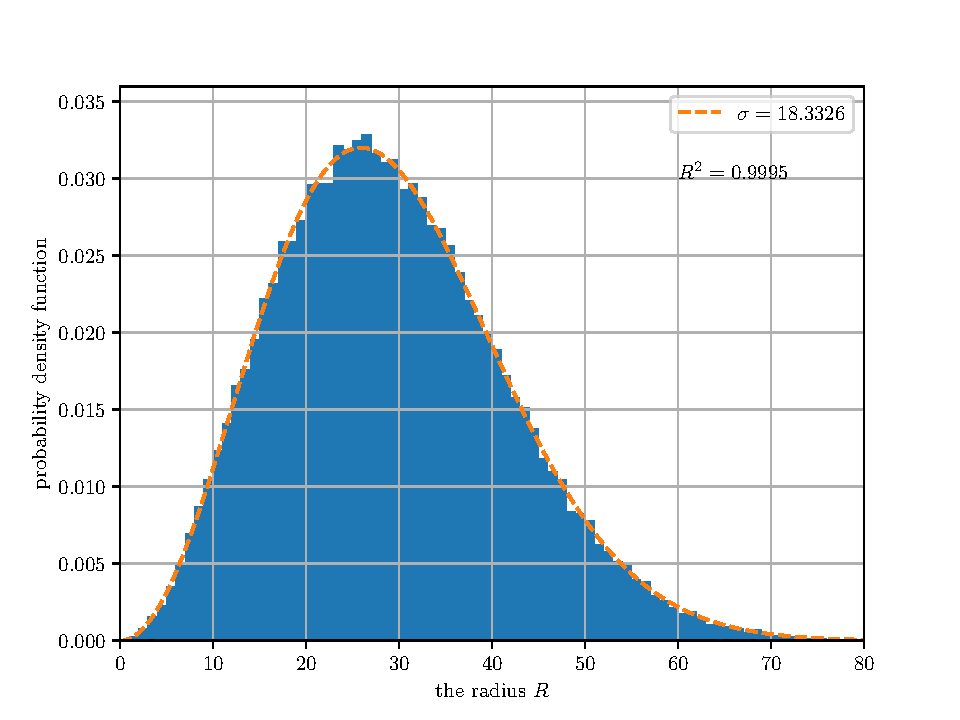
\includegraphics[width=\linewidth]{figure_2_1.pdf}
		\caption{}
	\end{subfigure}
	\begin{subfigure}[!b]{0.495\textwidth}
		\centering
		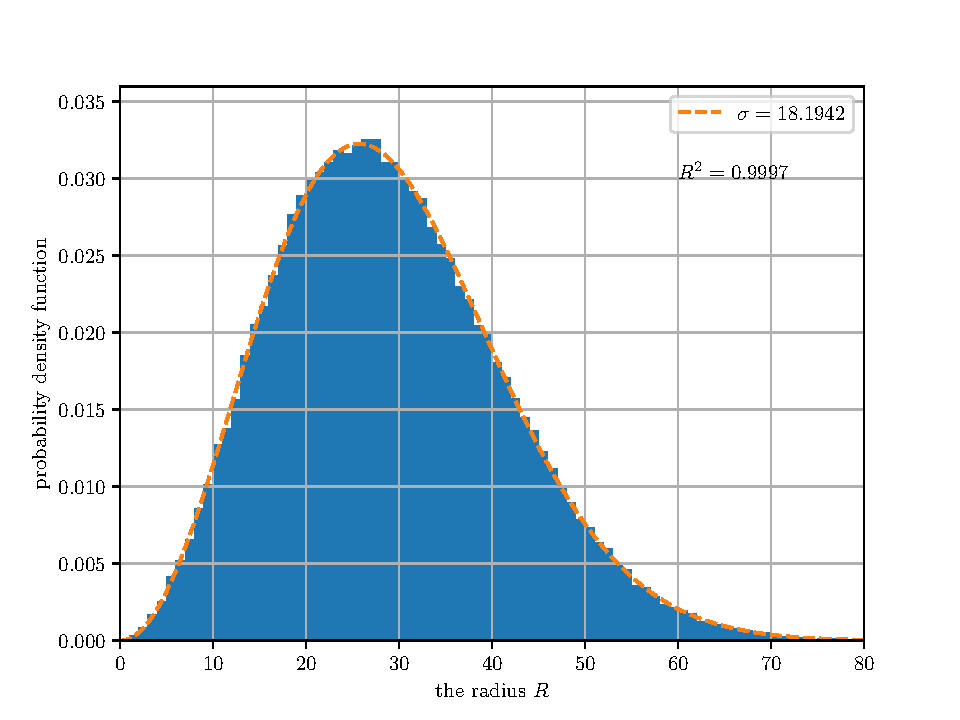
\includegraphics[width=\linewidth]{figure_2_2.pdf}
		\caption{}
	\end{subfigure}
	\caption{the radius distributions for three types of 3D random walk: (a) spherical; (b) spherical volume; (c) Gaussian.}
	\label{fig:random_walks_in_3d}
\end{figure}

% ----------------------------------------------------------------------------------------
%	PROBLEM 3
%----------------------------------------------------------------------------------------

\section{Brownian motors and ratchets}

We are unable to solve this task.\par

%----------------------------------------------------------------------------------------

\end{document}
